\section{Benchmarking and stress testing} \label{chap:Benchmarking}
In this chapter, we present how tests and benchmarks have been conducted, and describe the implementation. 
The goal with the stress tests and benchmarks is threefold: 
\begin{enumerate}
\item It helps us determine an upper limit of simultaneous users before response times renders a student unproductive.
\item It helps us determine the average pull time for clients using the Test Runner under different levels of stress.
\item It helps us helps good configurations for the Test Runner system
\item It helps us establish different implementations of the backend regresses in terms of response times.
\end{enumerate}
We used BenchmarkDotNet to conduct the benchmarks (see chapter \ref{chap:preliminaries}) and defined three components used solely for the benchmarks:
a client component simulating possible Test Runner client behavior, a Benchmark component responsible for orchestrating benchmarks for different Test Runner versions, and a test component ensuring that the client component can contact the Test Runner before running the benchmarks.

\subsection{Orchestration and Test Runner parameterization}
The benchmark and test components are managed in their own Docker containers, and are connected to a network enabling communication between them and the container hosting the Test Runner. 
Information necessary to establish the connection between Test Runner and other components are defined as environmental constants for the containers, and are passed into the relevant Dockerfiles describing the services.
These constants are then shared among the necessary components' Dockerfile, which then use the information to establish a connection to the Test Runner.
For instance, the environmental constants defining the network location of the Test Runner service is passed as arguments to the Dockerfiles for the tests and the benchmark, as these must both be able to contact the Test Runner service.
These environmental constants also allow easy adjustment of Test Runner implementing the Queue System without rebuilding the docker container.
These settings include the size of the queue system and the maximum number of threads the Test Runner can use to test the submitted Haskell code. 
It is also possible to adjust the time between sweeps and how long each Test Runner result should be stored in memory.
This makes it easy to experiment with different variables for the benchmarks and stress tests.  
The containers are orchestrated such that the benchmarks starts only if the test container exits successfully --- that is, all the tests pass successfully. 
Thus, wrongly configured containers do not result in misleading benchmark results.

\subsection{Selecting test parameters}
To achieve a varying degree of complexity for the submission content, several Haskell exercise solutions covering different concepts from course were selected, and Hspec tests based on the description of these problems were developed. 
The content of the code and test submitted to the backend can be seen in Appendix \ref{chap:TestCode}.
Each of the files covers a single topic from the course, including recursive type definitions and operations on such types, list comprehension, filtering of lists, and one containing a syntactical error.
After selecting a representative set of exercises for stress tests and benchmarks a simple operational profile was created, and from this behavioral variables were established: an expected maximum number of clients and different polling times for these clients.
To simulate different behavior of platform clients, classes representing clients were implemented, each representing a user for a different version of the platform.
These clients implement representations of the necessary behavioral variables, which are annotated using BenchmarkDotNet.
During stress testing, the BenchmarkDotNet framework creates all possible combinations of the implemented behavioral variables.
The underlying implementation of the client classes use an HTTP client.
To evaluate stress test and benchmark results of the developed Test Runner component, we first establish a baseline which we can compare the component to. 
To establish such baseline, we have stress tested and benchmarked a version of the Test Runner that utilize the Rocket crate but does not implement the Queue System. 
The benchmark for the baseline utilize the same parameterization as the benchmark for the queue system, but does not rely on polling the result after processing. 
We suspect that when the Test Runner experience stress, the single threaded approach will experience a form of starvation where all responses will take a long time to complete due to the asynchronous processing of the request, as each request will have to compete for CPU usage with all other requests.

\subsubsection{Ensuring simultaneous client submissions}
When performing stress tests one must ensure that the behavior stresses the system in a manner that is realistic, but on the edge of what is probable.
In the case of the Test Runner component, this means exposing it to numerous simultaneous requests. 
To ensure that all submissions to the component happens close to simultaneously, a method creating a number of actions and invoking them as tasks in close succession (see \ref{lst:TaskBuilder}, line 38 --- 54). 
When the actions are invoked, an inputted action is invoked with a CodeRunnerClient as input. 
We utilize this inputted action to send a code submissions requests and invoke start the clients in rapid succession.

\begin{lstlisting}[language=CSharp, escapechar=~, caption={C\# code showing the BuildClientTaskList method, which is used to build a number of actions which are executed simultaneously in a Task}, label={lst:TaskBuilder}]
public static class TaskBuilder
{
  public static IEnumerable<Task> BuildClientTaskList<T>(int count, Action<T> action)
      where T : CodeRunnerClient, new()
  {
    List<Action> clientActions = new(count);
    List<Task> tasks = new(count);
    
    for (int i = 0; i < count; i++)
    {
        T client = new();
        clientActions.Add(() => action.Invoke(client));
    }

    foreach (Action clientAction in clientActions)
    {
        tasks.Add(Task.Run(clientAction));
    }
    return tasks;
  }
}
\end{lstlisting}

\subsubsection{Baseline benchmark implementation}
The baseline benchmarks seen in listing \ref{lst:baselineBench} is executed multiple times for all combinations of code submissions and number of clients.
The benchmark itself measures the time it takes for all clients to post the code submission and receive an HTTP response with status code 200.
If just one of the submissions cannot be processed an exception is thrown, and the benchmark stops.
It utilizes the BuildClientTaskList method seen in listing \ref{lst:baselineBench}.
\begin{lstlisting}[language=CSharp, escapechar=~, caption={C\# code showing the implementation of the benchmark for the baseline}, label={lst:baselineBench}]
// Attributes excluded
public class RocketBenchmarks
{
    [Params(10, 20, 50, 100)] 
    public int NumberOfRequests { get; set; }
    [ParamsSource(nameof(CodeSubmissions))]
    public CodeSubmission CodeSubmission { get; set; }
    public static IEnumerable<CodeSubmission> CodeSubmissions => CodeLoader.Load();

    [Benchmark]
    public void PostAndWaitForResponseReceived()
    {
      IEnumerable<Task> clientActions = TaskBuilder.BuildClientTaskList<CodeRunnerClient>(NumberOfRequests,
        client => client.Post(CodeSubmission)
        .Result.EnsureSuccessStatusCode());
        
      Task.WhenAll(clientActions).Wait();
    }
}
\end{lstlisting}

\subsubsection{Queue system benchmark implementation}
The benchmark for the queue system seen on listing \ref{lst:queueSystemBench} is similar to the one in listing \ref{lst:baselineBench}, as it utilize the method from listing \ref{lst:TaskBuilder} and the parameterization attributes from BenchmarkDotNet.
However, the internal implementation of the client varies, as it needs to pull the results of the Test Runner after making an initial request.
Therefore, an additional parameter for the benchmark is introduced to examine how often a client should try to pull for a result.
Best case pull time needs to be established to compare it with the baseline component. 
However, due to the nature of remote communication using the internet it may be necessary to establish which polling times to avoid rather than which gives the best average response times, since the benchmarks does not consider the physical distance between client and server.
\begin{lstlisting}[language=CSharp, escapechar=~, caption={C\# code showing the implementation of the benchmark for the backend with the Queue System }, label={lst:queueSystemBench}]
// Attributes excluded
public class TicketedCodeRunnerBenchmark
{
    [Params(0.5, 1.0, 2.0, 3.0)] 
    public double PollTime { get; set; }
    [Params(10, 20, 50, 100)] 
    public int NumberOfRequests { get; set; }
    [ParamsSource(nameof(CodeSubmissions))] 
    public CodeSubmission CodeSubmission { get; set; }
    public static IEnumerable<CodeSubmission> CodeSubmissions => CodeLoader.Load();

    [Benchmark]
    public void PostAndWaitForAllResultsFetched()
    {
      TimeSpan timeBetweenPulls = TimeSpan.FromSeconds(PollTime);
      IEnumerable<Task> clientActions = TaskBuilder.BuildClientTaskList<CodeRunnerQueueClient>(NumberOfConcurrentRequests, 
        client => client.PostAndGetHaskellResultTask(CodeSubmission.code, CodeSubmission.test, timeBetweenPulls));

      Task.WhenAll(clientActions).Wait();
    }
}
\end{lstlisting}

\subsection{Results}
In this section, results of the combined stress tests and benchmarks are presented.
First, the configuration of the stress tests are described followed by a presentation of the results of the initial Test Runner benchmark results. These results will be used to compare the Test Runner using the Queue System with the baseline.  

\subsection{Configuration}
The baseline uses a single thread to test the submitted Haskell code, thus no parameterization for this version of the Test Runner is necessary.
Benchmarks for the Test Runner implementing the Queue System is configured such that the number of threads and the queue size varies by five. 
All stress tests and benchmarks are run on computers with an AMD EPYC Processor (with IBPB), four CPUs, four logical cores, and four physical cores.
The computers used for the benchmarks use UBUNTU 20.04 as the operating system and have 32GB of RAM.
All stress tests begins with a warm-up phase, where BenchmarkDotNet sends ten consecutive submissions to the Test Runner. 
Then, for each combination of parameters (number of requests, code submission, and polling times the stress test is timed and repeated 40 times.
This whole process is repeated five times to ensure outliers become noise.

\subsection{Baseline}
The baseline for all other benchmarks is a Test Runner implemented using Rocket. 
The baseline application uses only a single thread to handle all code submissions, giving us estimation on to what degree an implementation using Axum and the Queue System improves the overall response time of the platform.

\begin{figure}
  \centering
  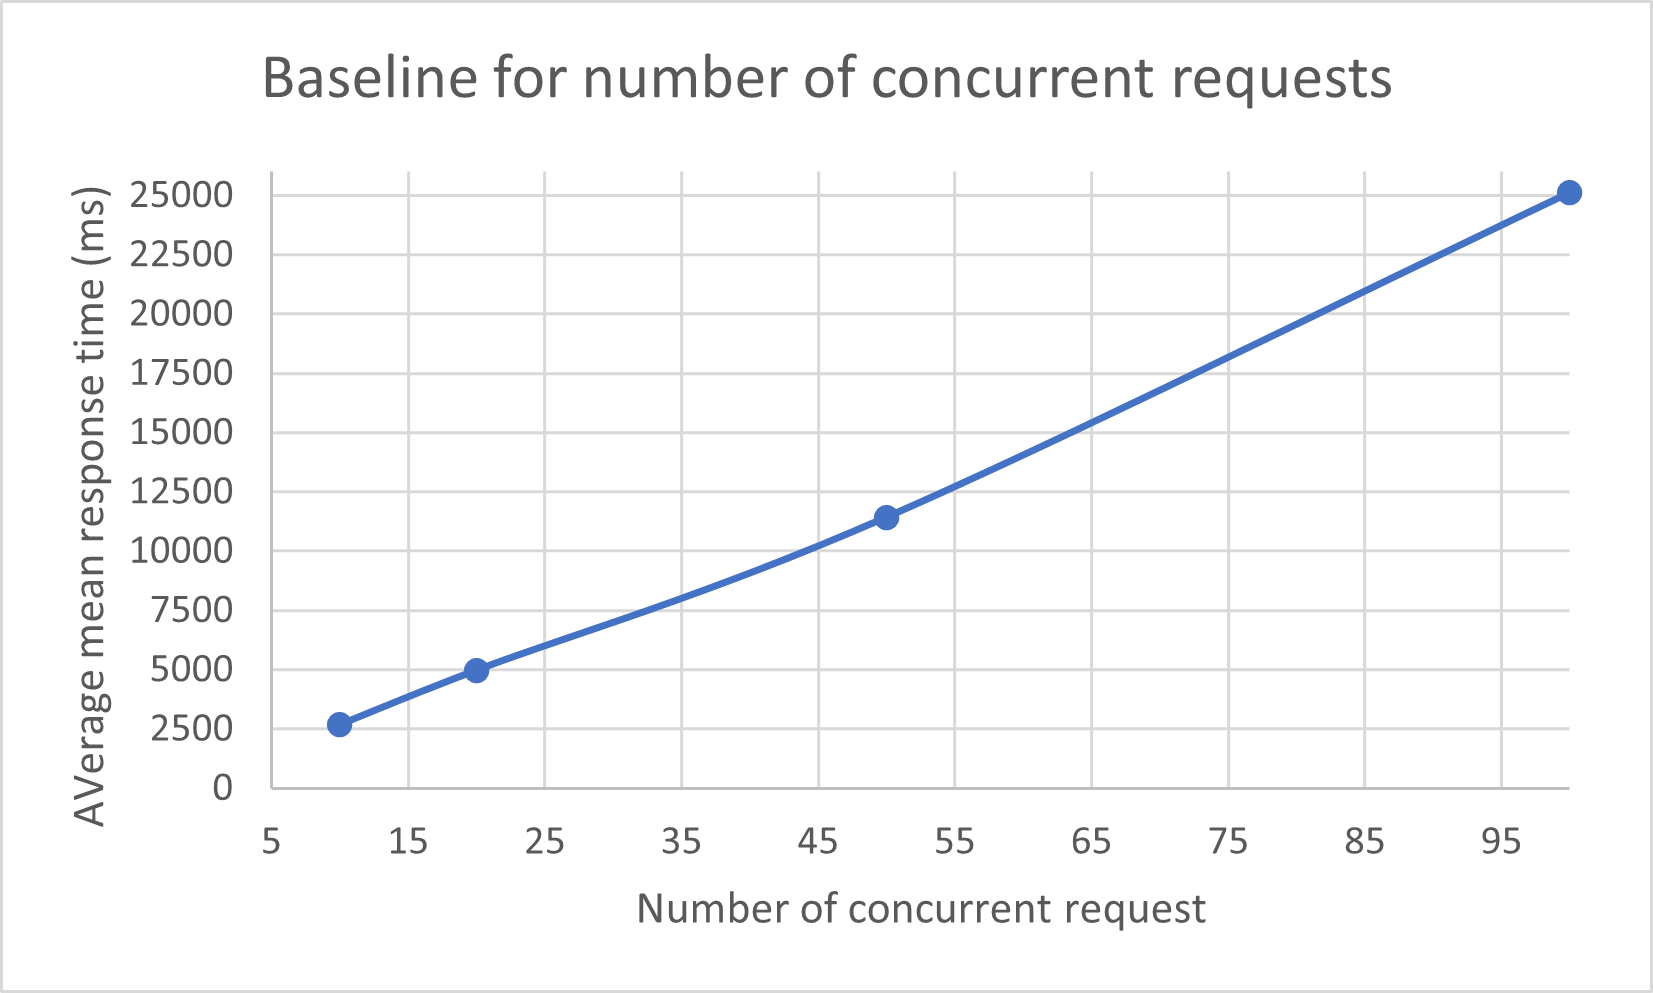
\includegraphics[scale=0.80]{images/baseline.png}
  \caption{The average mean time per request for the baseline Test Runner, disregarding the code submission}
  \label{fig:baseline}
\end{figure}
Figure \ref{fig:baseline} shows the average mean response time per number of requests for the baseline.
We expect the response time to increase linearly with the number of requests due to one request being handled at a time, and see on Figure \ref{fig:baseline} that this is the case.
The results for the benchmark of the baseline was examined further to see whether some code requests was much slower to process than others (see \ref{chap:AdditionalPlots}). 
We found that only one submission could be considered a direct outlier: namely the code submission containing syntactical errors.
This submission was faster to process, likely due to the exercise solution never being executed.


\subsection{Queue system}
\begin{figure}[!tbp]
  \begin{minipage}[t]{0.4\textwidth}
    \centering
    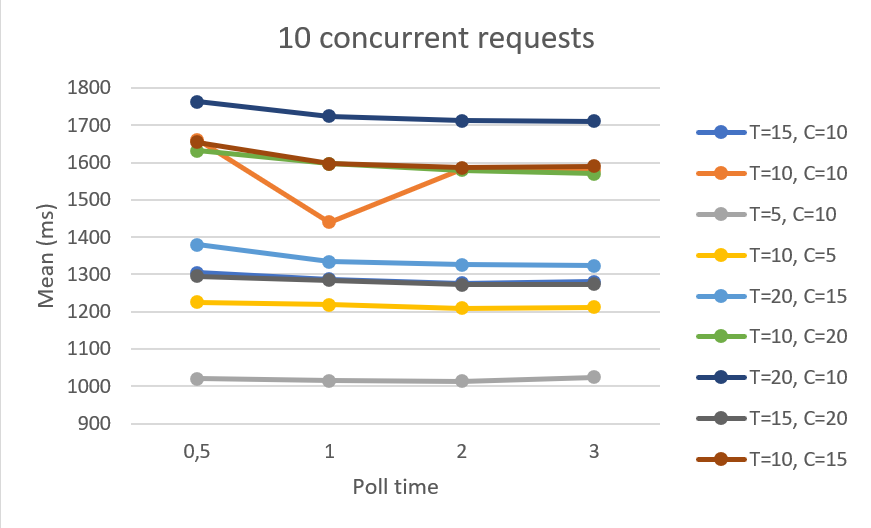
\includegraphics[scale=0.65]{images/10.png}
    \caption{Mean response time for handling 10 simultaneous client requests for different polling times and Test Runner configurations}
    \label{fig:resultstart}
  \end{minipage}
  \hfill
  \begin{minipage}[t]{0.4\textwidth}
    \centering
    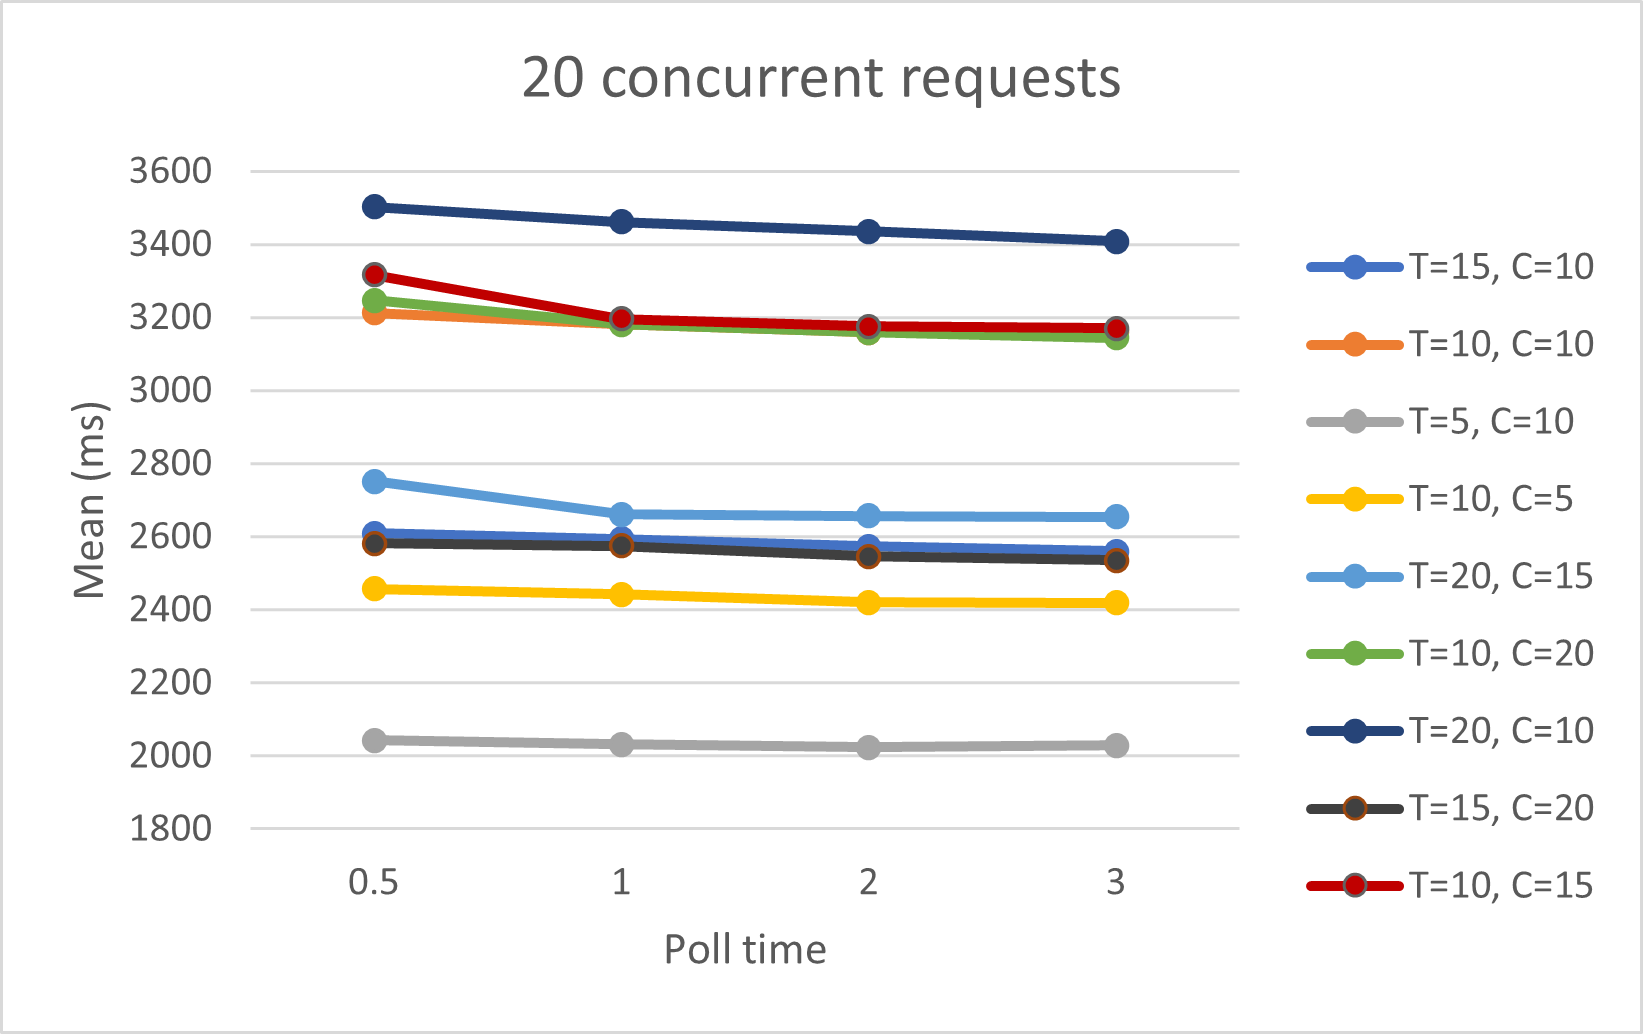
\includegraphics[scale=0.65]{images/20.png}
    \caption{Mean response time for handling 20 simultaneous client requests for different polling times and Test Runner configurations}
  \end{minipage}
  \begin{minipage}[t]{0.4\textwidth}
    \centering
    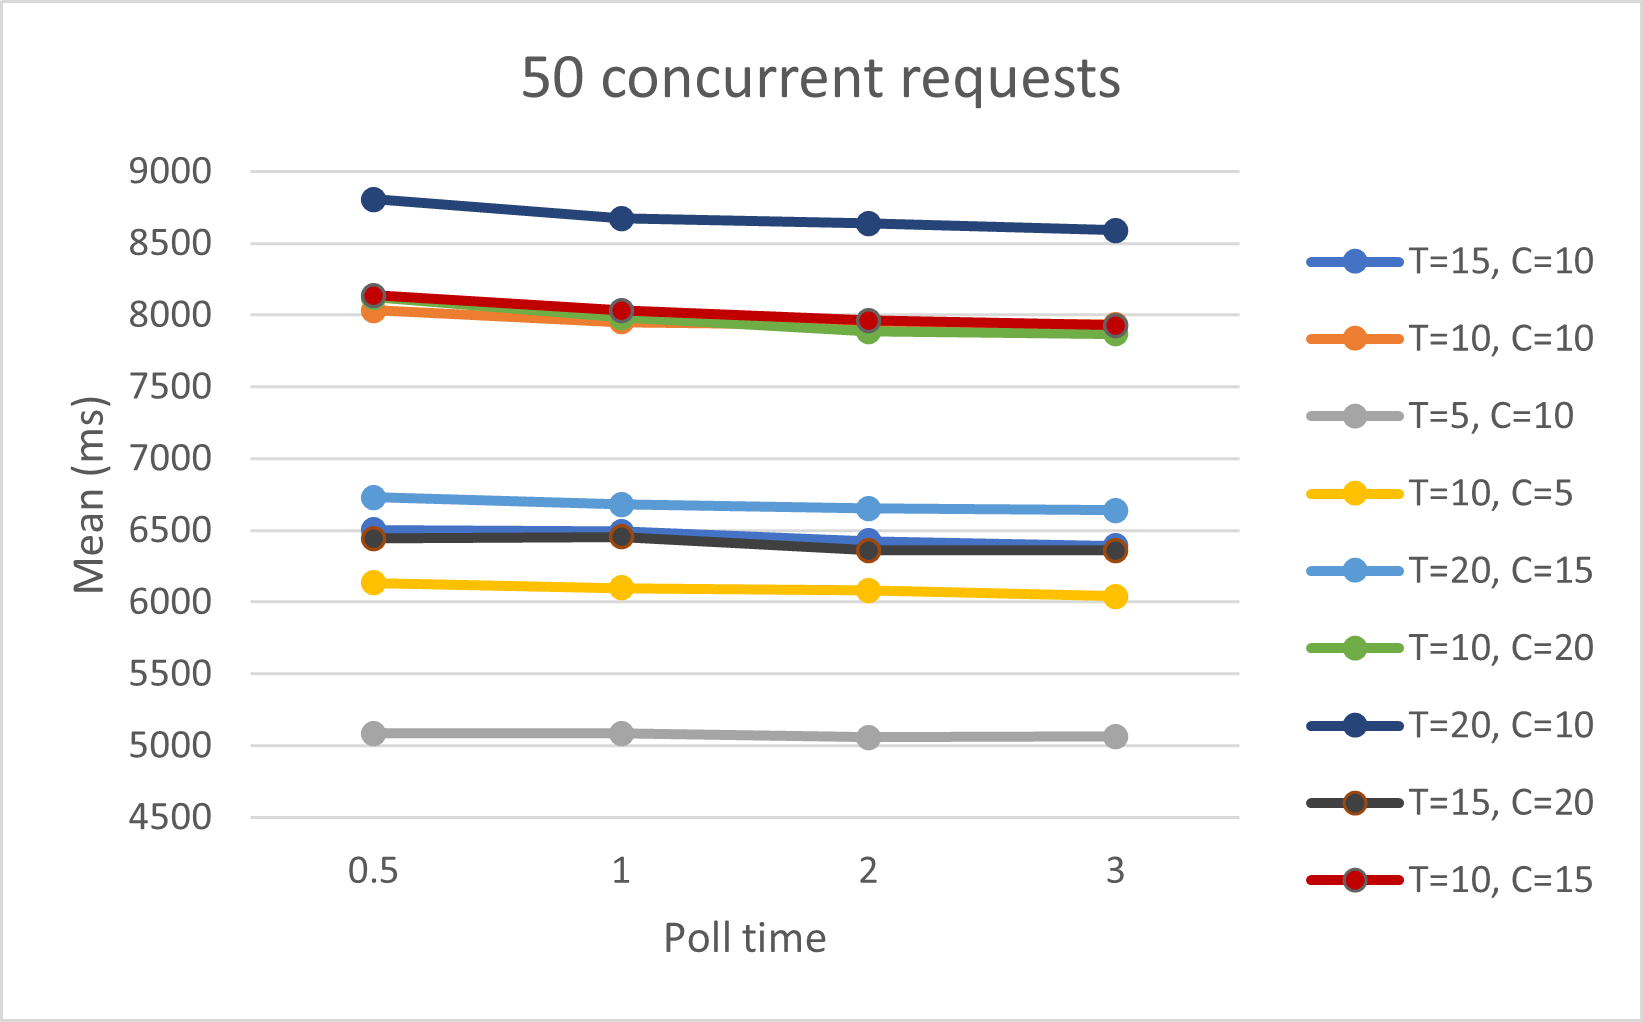
\includegraphics[scale=0.65]{images/50.png}
    \caption{Mean response time for handling 50 simultaneous client requests for different polling times and Test Runner configurations}
  \end{minipage}
  \hfill
  \begin{minipage}[t]{0.4\textwidth}
    \centering
    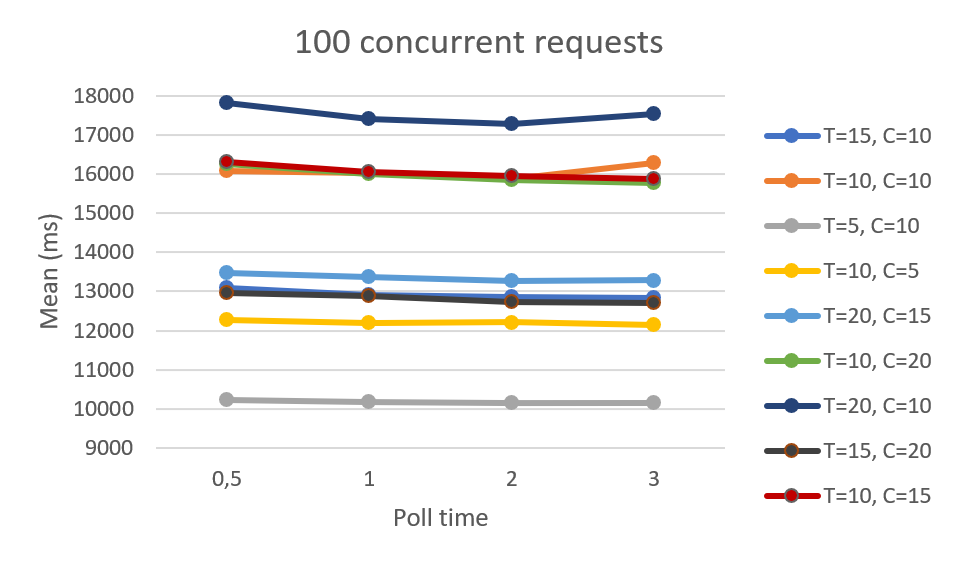
\includegraphics[scale=0.65]{images/100.png}
    \caption{Mean response time for handling 100 simultaneous client requests for different polling times and Test Runner configurations}
    \label{fig:resultEnd}
  \end{minipage}
\end{figure}

Figures \ref{fig:resultstart} --- \ref{fig:resultEnd} shows mean response time of benchmarking the Test Runner implementing the Queue System with different queue size, number of threads, and with clients having varying polling times. For each plot line T denotes the maximum number of threads allowed for testing client submissions and C the maximum capacity of the channels. 
All the benchmarks shown in figures \ref{fig:resultstart} --- \ref{fig:resultEnd} sweep the result queue every ten seconds, and remove Test Runner results older than 90 seconds. 
We see that a Test Runner with Queue System configured to have a maximum capacity of ten and a maximum of five threads surpasses all other configurations in terms of speed, regardless of the client pull time. 
Compared to the baseline shown on figure \ref{fig:baseline}, it is vastly superior, requiring only a third of the time responding to 100 simultaneous requests. 
Since a configuration of a Test Runner with five threads and with a channel capacity of ten yields such good results, we examine similar configurations to find a closer estimate to optimal configuration for this particular computer. 